\documentclass[conference]{IEEEtran}

\usepackage{cite}
\usepackage{amsmath,amssymb,amsfonts}
\usepackage{algorithmic}
\usepackage{graphicx}
\usepackage{textcomp}
\usepackage{xcolor}
\usepackage{booktabs}
\usepackage{multirow}
\usepackage{listings}
\usepackage{tikz}
\usetikzlibrary{shapes.geometric, arrows.meta, positioning, fit, calc,
                 shadows.blur, decorations.markings, backgrounds}
\usepackage{pgfplots}
\pgfplotsset{compat=1.18}
\usepgfplotslibrary{colorbrewer}
\usepackage{hyperref}
\usepackage{balance}

\lstdefinelanguage{SystemVerilog}{
  morekeywords={module, endmodule, always, begin, end, if, else, case,
    endcase, property, endproperty, assert, assume, posedge, negedge,
    logic, reg, wire, input, output, initial, default, assign},
  sensitive=true,
  morecomment=[l]{//},
  morecomment=[s]{/*}{*/},
  morestring=[b]",
}
\lstset{
  language=SystemVerilog,
  basicstyle=\footnotesize\ttfamily,
  keywordstyle=\bfseries\color{blue!70!black},
  commentstyle=\itshape\color{green!50!black},
  stringstyle=\color{red!60!black},
  numbers=left,
  numberstyle=\tiny\color{gray},
  numbersep=5pt,
  frame=single,
  breaklines=true,
  captionpos=b,
  tabsize=2,
  xleftmargin=1.5em,
  framexleftmargin=1.5em,
}

\def\BibTeX{{\rm B\kern-.05em{\sc i\kern-.025em b}\kern-.08em T\kern-.1667em\lower.7ex\hbox{E}\kern-.125emX}}

\begin{document}

\title{VISTA: Verification using Intelligent Systems for Test Automation --- LLM-Driven SystemVerilog Assertion Generation with Formal Validation}

\author{
\IEEEauthorblockN{Asad Ali\IEEEauthorrefmark{1}, Sheikh Abbas\IEEEauthorrefmark{1}, Mian Arqam\IEEEauthorrefmark{1}, Dr.\ Fahad Bin Muslim\IEEEauthorrefmark{2}}
\IEEEauthorblockA{\IEEEauthorrefmark{1}Department of Computer Engineering,\\
Ghulam Ishaq Khan Institute of Engineering Sciences and Technology, Topi, Pakistan\\
Email: \{asadnaeem4817, sheikhabbas, mianarqam\}@giki.edu.pk}
\IEEEauthorblockA{\IEEEauthorrefmark{2}Department of Computer Engineering,\\
Ghulam Ishaq Khan Institute of Engineering Sciences and Technology, Topi, Pakistan\\
Email: fahad.muslim@giki.edu.pk}
}

\maketitle

% ============================================================
\begin{abstract}
Formal verification is critical for ensuring the correctness of RTL designs, yet writing SystemVerilog Assertions~(SVA) manually is time-consuming, error-prone, and demands deep domain expertise. We present \textbf{VISTA} (Verification using Intelligent Systems for Test Automation), an end-to-end framework that automatically generates SVA directly from RTL code snippets using a fine-tuned LLaMA~3.1~(8B) large language model. The model is trained with QLoRA-based parameter-efficient fine-tuning on 19{,}000 RTL--SVA pairs from the VERT dataset, incorporating clock-domain and synchronization metadata. Because benchmark datasets provide RTL fragments rather than complete modules, VISTA introduces a \emph{dynamic RTL wrapping template} that transforms conditional snippets into synthesizable module-level descriptions with proper signal declarations, clock semantics, and reset initialization, making them directly consumable by the open-source formal verification tool SymbiYosys. A dedicated post-processing pipeline extracts property blocks from raw LLM output, converts temporal SVA operators into Yosys-compatible immediate assertions, and applies greedy syntax filtering. Evaluated on 100 VERT test samples, VISTA achieves a \textbf{99\% formal verification pass rate}, \textbf{99.1\% token-level Jaccard similarity} to gold-standard assertions, \textbf{89\% exact match rate}, and \textbf{100\% syntactic validity}. These results demonstrate that domain-specific LLM fine-tuning, combined with robust wrapper generation and assertion post-processing, can substantially automate hardware assertion-based verification.
\end{abstract}

\begin{IEEEkeywords}
Hardware Verification, SystemVerilog Assertions, Large Language Models, RTL-to-SVA Generation, Formal Verification, QLoRA Fine-Tuning, SymbiYosys
\end{IEEEkeywords}

% ============================================================
\section{Introduction}
\label{sec:intro}

Verification consumes an estimated 60--70\% of the total effort in modern System-on-Chip~(SoC) design cycles~\cite{foster2015trends}. SystemVerilog Assertions~(SVA), defined by the IEEE~1800-2023 standard~\cite{ieee1800}, enable designers to formally specify expected design behavior at the register-transfer level~(RTL). Despite their effectiveness, manually authoring SVA requires significant expertise in both the design under test and the assertion language, making the process a persistent bottleneck.

Prior approaches to assertion generation broadly fall into three categories: (i)~static analysis methods such as GoldMine~\cite{goldmine} and HARM~\cite{harm}, which mine properties from simulation traces but struggle with temporal complexity; (ii)~specification-driven LLM methods such as Spec2Assertion~\cite{spec2assertion} and AssertLLM~\cite{assertllm}, which require natural-language specifications that are often incomplete; and (iii)~knowledge-graph approaches like AssertionForge~\cite{assertionforge}, which depend on design-intent documentation. A common limitation is the reliance on external artifacts beyond the RTL itself.

In this work, we introduce \textbf{VISTA}, a framework that generates SVA \emph{directly from RTL code} without requiring natural-language specifications or simulation traces. Our contributions are:

\begin{enumerate}
    \item A fine-tuned LLaMA~3.1~(8B) model trained on 19{,}000 RTL--SVA pairs using QLoRA~\cite{qlora} with Unsloth~\cite{unsloth} optimizations, achieving efficient training on a single GPU with under 6\,GB VRAM.
    \item A \emph{dynamic RTL wrapping template} that converts conditional RTL fragments into complete, formally verifiable modules with inferred signal declarations, width annotations, and clock/reset semantics.
    \item A multi-stage \emph{assertion post-processing pipeline} that extracts SVA property blocks, converts temporal operators to Yosys-compatible immediate assertions, sanitizes expressions, and applies greedy syntax filtering via Yosys.
    \item A comprehensive evaluation on 100 VERT~\cite{vert} samples demonstrating 99\% formal pass rate, 99.1\% Jaccard similarity, and 89\% exact match with gold assertions.
\end{enumerate}

% ============================================================
\section{Related Work}
\label{sec:related}

\textbf{Traditional assertion mining.}
GoldMine~\cite{goldmine} applies data-flow analysis and simulation-based mining to extract candidate assertions from RTL designs. HARM~\cite{harm} extends this with temporal pattern recognition. Both methods generate large sets of weak candidate assertions that require substantial manual pruning and cannot capture complex sequential behaviors.

\textbf{Specification-driven LLM approaches.}
Spec2Assertion~\cite{spec2assertion} translates natural-language protocol specifications into SVA by decomposing them into cause--effect structures. AssertLLM~\cite{assertllm} augments specifications with waveform traces to improve assertion quality. AssertionForge~\cite{assertionforge} employs knowledge graphs to reconcile design intent with RTL implementation. While effective, these methods depend on the availability and completeness of natural-language specifications---a significant limitation in practice.

\textbf{Benchmark-driven evaluation.}
AssertionBench~\cite{assertionbench} provides formally verified Verilog modules with reference assertions for evaluating LLM-based generation. Studies using this benchmark demonstrate that domain-fine-tuned models like LLaMA~3.1 variants outperform general-purpose LLMs~\cite{enhancing_llm_hw}.

\textbf{The VERT dataset.}
VERT~\cite{vert} provides 20{,}000 RTL--SVA pairs for training assertion-generation models. However, the dataset consists of RTL \emph{fragments} (conditional blocks, case statements) rather than complete modules, making direct formal verification impossible without a wrapper layer.

VISTA distinguishes itself by: (1)~generating assertions directly from RTL without external specifications; (2)~introducing a dynamic wrapper that enables formal verification of fragment-level RTL; and (3)~providing an automated end-to-end pipeline from raw RTL to verified assertions using the open-source SymbiYosys~\cite{symbiyosys} toolchain.

% ============================================================
\section{Proposed Methodology}
\label{sec:methodology}

Fig.~\ref{fig:pipeline} illustrates the VISTA pipeline, which comprises four stages: prompt construction, LLM inference, assertion post-processing, and formal verification.

\begin{figure*}[t]
\centering
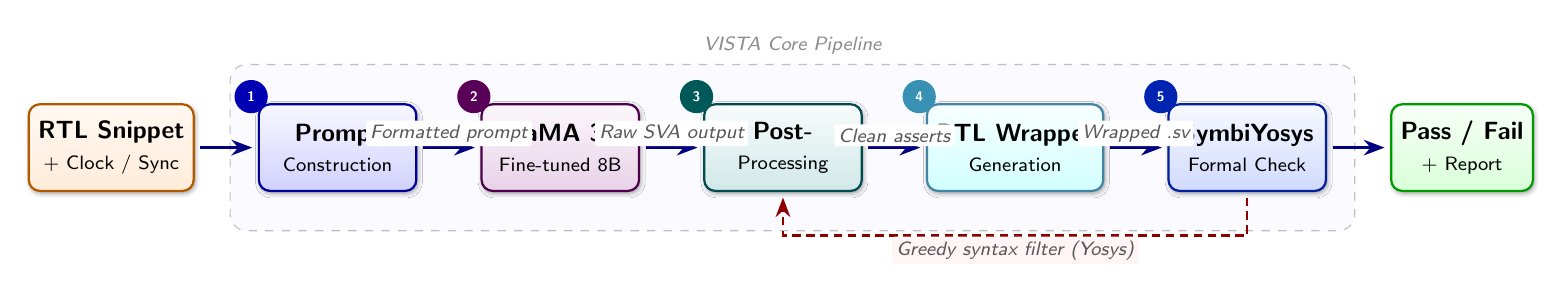
\begin{tikzpicture}[
    node distance=0.35cm and 0.55cm,
    >=Stealth,
    % --- Professional node styles ---
    inputnode/.style={
        draw=orange!70!black, line width=0.8pt, rounded corners=4pt,
        fill=orange!8, top color=orange!5, bottom color=orange!15,
        minimum width=1.8cm, minimum height=1.1cm,
        align=center, font=\small\sffamily,
        blur shadow={shadow blur steps=6, shadow xshift=0.5pt, shadow yshift=-0.8pt}
    },
    stagenode/.style={
        draw=#1!60!black, line width=0.8pt, rounded corners=4pt,
        fill=#1!6, top color=#1!3, bottom color=#1!18,
        minimum width=2.0cm, minimum height=1.1cm,
        align=center, font=\small\sffamily,
        blur shadow={shadow blur steps=6, shadow xshift=0.5pt, shadow yshift=-0.8pt}
    },
    stagenode/.default=blue,
    outputnode/.style={
        draw=green!60!black, line width=0.8pt, rounded corners=4pt,
        fill=green!6, top color=green!3, bottom color=green!15,
        minimum width=1.8cm, minimum height=1.1cm,
        align=center, font=\small\sffamily,
        blur shadow={shadow blur steps=6, shadow xshift=0.5pt, shadow yshift=-0.8pt}
    },
    % --- Arrow styles ---
    mainflow/.style={->, thick, color=blue!50!black, line width=1pt,
        shorten >=2pt, shorten <=2pt},
    feedback/.style={->, densely dashed, thick, color=red!55!black, line width=0.9pt,
        shorten >=2pt, shorten <=2pt},
    datalbl/.style={font=\scriptsize\sffamily\itshape, text=black!65, fill=white,
        inner sep=1.5pt, rounded corners=1pt},
    stagelbl/.style={font=\tiny\sffamily\bfseries, text=black!50},
]

% ---- Nodes (left to right flow) ----
\node[inputnode] (input) {\textbf{RTL Snippet}\\{\scriptsize + Clock / Sync}};

\node[stagenode, right=0.8cm of input] (prompt) {\textbf{Prompt}\\{\scriptsize Construction}};

\node[stagenode=violet, right=0.8cm of prompt] (llm) {\textbf{LLaMA 3.1}\\{\scriptsize Fine-tuned 8B}};

\node[stagenode=teal, right=0.8cm of llm] (post) {\textbf{Post-}\\{\scriptsize Processing}};

\node[stagenode=cyan, right=0.8cm of post] (wrap) {\textbf{RTL Wrapper}\\{\scriptsize Generation}};

\node[stagenode=blue!80!cyan, right=0.8cm of wrap] (sby) {\textbf{SymbiYosys}\\{\scriptsize Formal Check}};

\node[outputnode, right=0.8cm of sby] (result) {\textbf{Pass / Fail}\\{\scriptsize + Report}};

% ---- Stage number badges ----
\foreach \nd/\num/\col in {prompt/1/blue, llm/2/violet, post/3/teal, wrap/4/cyan, sby/5/blue!80!cyan}{
    \node[circle, fill=\col!70!black, text=white, font=\tiny\sffamily\bfseries,
          inner sep=1.2pt, minimum size=12pt,
          above left=-2pt and -2pt of \nd.north west] {\num};
}

% ---- Main flow arrows with data labels ----
\draw[mainflow] (input)  -- (prompt);
\draw[mainflow] (prompt) -- (llm)  node[datalbl, midway, above] {Formatted prompt};
\draw[mainflow] (llm)    -- (post) node[datalbl, midway, above] {Raw SVA output};
\draw[mainflow] (post)   -- (wrap) node[datalbl, midway, above] {Clean asserts};
\draw[mainflow] (wrap)   -- (sby)  node[datalbl, midway, above] {Wrapped .sv};
\draw[mainflow] (sby)    -- (result);

% ---- Greedy feedback loop (below) ----
\draw[feedback]
    (sby.south) -- ++(0, -0.55)
    -| node[datalbl, pos=0.25, below, fill=red!4]
       {Greedy syntax filter (Yosys)}
    (post.south);

% ---- Background grouping box ----
\begin{scope}[on background layer]
\node[draw=black!25, dashed, rounded corners=6pt, fill=blue!2,
      fit=(prompt)(llm)(post)(wrap)(sby),
      inner xsep=10pt, inner ysep=14pt,
      label={[font=\scriptsize\sffamily\itshape, text=black!45]above:{VISTA Core Pipeline}}
     ] {};
\end{scope}

\end{tikzpicture}
\caption{VISTA pipeline architecture. RTL snippets with clock/synchronization metadata enter the five-stage pipeline: (1)~prompt construction aligning input to the training format, (2)~LLM inference via the fine-tuned LLaMA~3.1 model, (3)~multi-step post-processing converting SVA temporal operators to Yosys-compatible immediate assertions, (4)~dynamic RTL wrapper generation with signal inference and clock-aware structuring, and (5)~bounded model checking with SymbiYosys. A greedy feedback loop (dashed) filters syntactically invalid assertions by re-invoking Yosys during post-processing.}
\label{fig:pipeline}
\end{figure*}

\subsection{Stage 1: Prompt Construction}
Each RTL sample is formatted using a structured prompt template aligned with the model's training format:
\begin{quote}
\small\ttfamily
\#\#\# Instruction:\\
You are a hardware verification assistant. Given the RTL code and the synchronous/clock info, produce the formal assertion(s) that verify the behaviour.\\[2pt]
Synchronous: \{sync\}\\
Clock: \{clock\}\\[2pt]
Code:\\
\{rtl\_code\}\\[2pt]
OUTPUT (Assertions):\\[2pt]
\#\#\# Response:
\end{quote}
Prompt--training alignment is critical: mismatches between evaluation and training prompt formats caused a 75\% drop in assertion yield during development (Section~\ref{sec:ablation}).

\subsection{Stage 2: LLM Inference}
The fine-tuned LLaMA~3.1~(8B) model generates SVA property blocks in response to the prompt. Inference uses greedy decoding with a maximum of 512 new tokens to accommodate complex multi-branch RTL designs that require multiple assertions.

\subsection{Stage 3: Assertion Post-Processing}
\label{sec:postproc}
Raw LLM output undergoes a multi-step transformation:
\begin{enumerate}
    \item \textbf{Region extraction}: The response region after \texttt{\#\#\# Response:} is isolated.
    \item \textbf{Property block parsing}: Regex-based extraction of \texttt{property}$\ldots$\texttt{endproperty} blocks, handling both semicolon and colon delimiters after property names.
    \item \textbf{Temporal-to-immediate conversion}: SVA temporal operators (\texttt{|->}, \texttt{|=>}, \texttt{\#\#N}) are converted to Yosys-compatible Boolean immediate assertions. An implication \texttt{A |-> B} becomes \texttt{assert((!A) || B)}.
    \item \textbf{Expression sanitization}: Clock qualifiers (\texttt{@(posedge clk)}), \texttt{disable iff} clauses, and system functions (\texttt{\$past}, \texttt{\$rose}) are stripped or replaced with safe constants.
    \item \textbf{Greedy syntax filtering}: Each assertion is individually validated by Yosys; only assertions that pass parsing are retained.
\end{enumerate}

\subsection{Stage 4: Dynamic RTL Wrapper}
\label{sec:wrapper}
A central challenge is that benchmark datasets (e.g., VERT) provide conditional RTL fragments, not complete modules. VISTA addresses this with a dynamic wrapper generator:
\begin{itemize}
    \item \textbf{Signal inference}: Identifiers are extracted from both RTL code and assertion expressions, filtered against a comprehensive set of 80+ Verilog/SystemVerilog keywords, and declared as \texttt{logic [31:0]} signals (or inferred widths from RTL declarations).
    \item \textbf{Clock-aware structuring}: For synchronous designs, RTL and assertions are placed in matching clocked \texttt{always} blocks; for combinational designs, assertions are embedded in the same \texttt{always @*} block as the RTL to ensure correct signal evaluation order.
    \item \textbf{State initialization}: All signals are initialized to zero in an \texttt{initial} block. Synchronous wrappers use a \texttt{\_started} flag to skip assertions during the first clock cycle when signals are uninitialized.
\end{itemize}

Listing~\ref{lst:wrapper} shows a generated wrapper for a synchronous RTL fragment.

\begin{lstlisting}[caption={Generated wrapper for synchronous RTL with clocked assertion block.},label={lst:wrapper},float=t]
`timescale 1ns/1ps
module vert_formal_wrap;
  logic clk;
  logic rst;
  initial begin
    rst = 1'b0;
    sig_a = '0;  sig_b = '0;  out = '0;
  end
  logic [31:0] sig_a, sig_b, out;

  reg _started = 0;
  always @(posedge clk) begin
    // --- Original RTL fragment ---
    if (sig_a && sig_b) begin
      out <= sig_a + sig_b;
    end
    _started <= 1;
  end

  always @(posedge clk) begin
    if (_started) begin
      assume (!rst);
      assert ((!(sig_a && sig_b))
              || (out == sig_a + sig_b));
    end
  end
endmodule
\end{lstlisting}

% ============================================================
\section{Dataset and Training}
\label{sec:training}

\subsection{Dataset}
We use the VERT dataset~\cite{vert}, comprising 19{,}000 RTL--SVA pairs. Each sample contains: an RTL code fragment (conditional blocks, case statements, or nested control flow), one or more gold-standard SVA property blocks, a synchronous/asynchronous flag, and a clock specification (e.g., \texttt{posedge pll\_clk\_12}). The dataset covers a variety of RTL constructs including \texttt{if-else} chains, \texttt{case}/\texttt{casex} statements, nested conditionals, and reset-guarded logic. A 95/5 training/validation split is used.

\subsection{Model and Fine-Tuning}
We fine-tune Meta's LLaMA~3.1~(8B) using QLoRA~\cite{qlora} with the Unsloth~\cite{unsloth} optimization framework. Table~\ref{tab:training} summarizes the training configuration.

\begin{table}[t]
\centering
\caption{Training Configuration}
\label{tab:training}
\begin{tabular}{@{}ll@{}}
\toprule
\textbf{Parameter} & \textbf{Value} \\
\midrule
Base model & LLaMA 3.1 (8B) \\
Quantization & 4-bit (QLoRA) \\
LoRA rank ($r$) & 256 \\
LoRA alpha ($\alpha$) & 256 \\
LoRA dropout & 0.0 \\
Target modules & q, k, v, o, gate, up, down proj \\
Learning rate & $1 \times 10^{-4}$ \\
LR scheduler & Cosine \\
Batch size (effective) & 64 (micro=2, accum=32) \\
Epochs & 3 \\
Max sequence length & 4{,}096 tokens \\
Precision & BF16 \\
Hardware & NVIDIA RTX 4090 (24\,GB) \\
Optimizer & AdamW \\
VRAM usage & $<$6\,GB (with Unsloth) \\
\bottomrule
\end{tabular}
\end{table}

The high LoRA rank ($r=256$) was chosen to maximize the model's capacity to learn the structured mapping between RTL control flow and SVA property blocks. All seven attention and MLP projection matrices are adapted, providing broad coverage of the model's internal representations.

\subsection{Prompt Format}
Training samples use the format: \texttt{\#\#\# Instruction:} followed by the task description, synchronous/clock metadata, and RTL code, with the target SVA after \texttt{\#\#\# Response:}. The evaluation prompt template is identical to the training format, which proved critical for maximizing assertion yield (Section~\ref{sec:ablation}).

% ============================================================
\section{Evaluation Methodology}
\label{sec:eval}

\subsection{Test Set}
We evaluate on 100 held-out VERT samples spanning both synchronous (48 samples) and combinational (52 samples) designs with varying complexity (1--8 gold assertions per sample).

\subsection{Metrics}
We report five complementary metrics:

\begin{itemize}
    \item \textbf{Syntactic validity}: Percentage of cases where all generated assertions pass Yosys parsing (\texttt{read\_verilog -formal -sv}).
    \item \textbf{Formal pass rate}: Percentage of cases where SymbiYosys bounded model checking (BMC, depth~8) reports PASS.
    \item \textbf{Gold Jaccard similarity}: Token-level Jaccard coefficient between the set of generated assertion strings and the set of gold-standard assertions, averaged across all samples.
    \item \textbf{Exact match rate}: Percentage of samples achieving Jaccard $\geq 0.999$.
    \item \textbf{Assertion yield}: Percentage of samples where the model produces at least one non-trivial assertion.
\end{itemize}

\subsection{Formal Verification Setup}
Each test case is assembled into a complete module using the dynamic wrapper (Section~\ref{sec:wrapper}), paired with an SBY configuration file specifying BMC mode with the \texttt{smtbmc} engine, and executed via SymbiYosys~\cite{symbiyosys}. The tool reports PASS (no counterexample found within depth), FAIL (counterexample exists), or ERROR.

% ============================================================
\section{Results and Discussion}
\label{sec:results}

\subsection{Main Results}

Table~\ref{tab:results} presents the evaluation results across 100 VERT test samples.

\begin{table}[t]
\centering
\caption{VISTA Evaluation Results on 100 VERT Samples}
\label{tab:results}
\begin{tabular}{@{}lc@{}}
\toprule
\textbf{Metric} & \textbf{Result} \\
\midrule
Syntactic validity & 100/100 (100\%) \\
Formal verification pass & 99/100 (99\%) \\
Gold Jaccard (mean) & 0.991 \\
Exact match (Jaccard $\geq$ 0.999) & 89/100 (89\%) \\
Assertion yield & 100/100 (100\%) \\
Total assertions generated & 458 \\
Average assertions per case & 4.6 \\
Greedy-filtered assertions & 14 \\
\bottomrule
\end{tabular}
\end{table}

VISTA achieves 100\% syntactic validity across all 100 cases, indicating that the post-processing pipeline and greedy filter successfully normalize all LLM outputs into valid SystemVerilog. The 99\% formal pass rate demonstrates that the generated assertions are not only syntactically correct but also logically consistent with the RTL behavior. The single formal failure (Case~82) involves a \texttt{casex}-style bit pattern (\texttt{6'bx000x0}) where don't-care bits cause semantic mismatch under Yosys SMT equality checking---a tool limitation rather than a model error.

\subsection{Breakdown by Design Type}

Table~\ref{tab:breakdown} presents results stratified by synchronous vs.\ combinational designs.

\begin{table}[t]
\centering
\caption{Results by Design Type}
\label{tab:breakdown}
\begin{tabular}{@{}lccc@{}}
\toprule
\textbf{Type} & \textbf{Count} & \textbf{SBY Pass} & \textbf{Jaccard} \\
\midrule
Synchronous & 48 & 47/48 (98\%) & 0.990 \\
Combinational & 52 & 52/52 (100\%) & 0.993 \\
\midrule
\textbf{Overall} & \textbf{100} & \textbf{99/100 (99\%)} & \textbf{0.991} \\
\bottomrule
\end{tabular}
\end{table}

Combinational designs achieve a perfect 100\% pass rate because assertions are evaluated in the same \texttt{always @*} block as the RTL, guaranteeing that signal assignments precede assertion checks. Synchronous designs require the \texttt{\_started} flag mechanism to skip the uninitialized first cycle, yielding 98\% (the single failure being the \texttt{casex} edge case).

\subsection{Assertion Quality Analysis}

Fig.~\ref{fig:jaccard_dist} shows the distribution of per-sample Jaccard similarity scores.

\begin{figure}[t]
\centering
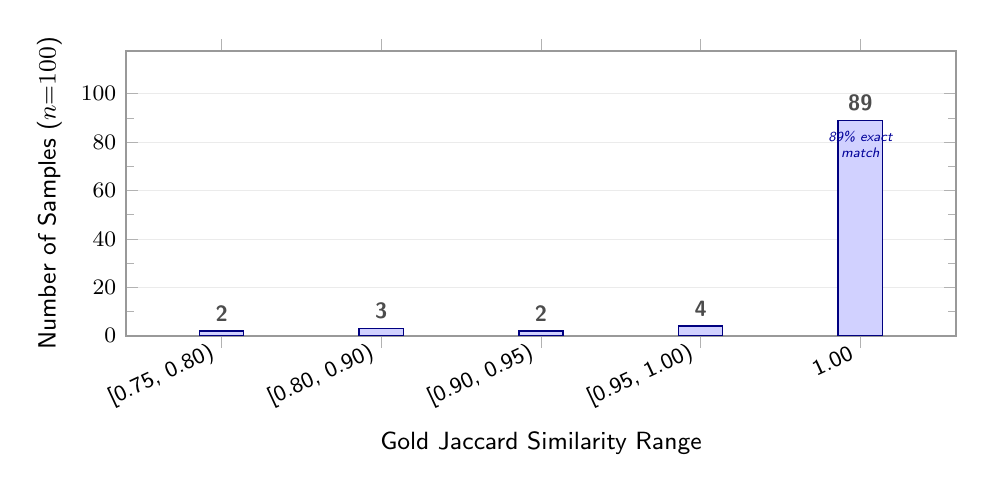
\begin{tikzpicture}
\begin{axis}[
    ybar,
    bar width=16pt,
    width=\columnwidth,
    height=5.2cm,
    xlabel={\small Gold Jaccard Similarity Range},
    ylabel={\small Number of Samples ($n{=}100$)},
    xlabel style={font=\sffamily},
    ylabel style={font=\sffamily},
    symbolic x coords={
        {[0.75, 0.80)},
        {[0.80, 0.90)},
        {[0.90, 0.95)},
        {[0.95, 1.00)},
        {1.00}
    },
    xtick=data,
    xticklabel style={rotate=25, anchor=east, font=\footnotesize\sffamily},
    yticklabel style={font=\footnotesize\sffamily},
    ymin=0, ymax=105,
    ytick={0, 20, 40, 60, 80, 100},
    minor y tick num=1,
    grid=major,
    grid style={draw=black!8, line width=0.3pt},
    ymajorgrids=true,
    xmajorgrids=false,
    nodes near coords,
    nodes near coords style={font=\footnotesize\sffamily\bfseries, color=black!70, above},
    point meta=explicit symbolic,
    enlarge x limits=0.15,
    enlarge y limits={upper, value=0.12},
    axis line style={draw=black!40, line width=0.5pt},
    tick style={draw=black!30},
    area legend,
    legend style={at={(0.03, 0.97)}, anchor=north west, font=\scriptsize\sffamily,
                  draw=black!20, fill=white, fill opacity=0.85},
]

% Gradient-colored bars: lighter for low counts, dark for the dominant bar
\addplot[
    fill=blue!18, draw=blue!50!black, line width=0.5pt,
] coordinates {
    ({[0.75, 0.80)}, 2) [2]
    ({[0.80, 0.90)}, 3) [3]
    ({[0.90, 0.95)}, 2) [2]
    ({[0.95, 1.00)}, 4) [4]
    ({1.00}, 89) [\textbf{89}]
};

% Highlight annotation for the dominant bar
\node[font=\tiny\sffamily\itshape, text=blue!60!black, align=center]
    at (axis cs:{1.00}, 79) {89\% exact\\match};

\end{axis}
\end{tikzpicture}
\caption{Distribution of token-level Gold Jaccard similarity scores across the 100-sample VERT test set. The distribution is heavily concentrated at 1.0 (exact match), with 89 samples achieving perfect overlap with gold-standard assertions. Only 2 samples fall below 0.80, differing in minor expression formatting rather than semantic content.}
\label{fig:jaccard_dist}
\end{figure}

The distribution is heavily right-skewed, with 89\% of samples achieving exact match and only 2 samples falling below 0.80. The non-exact cases typically differ in assertion ordering or minor expression formatting rather than semantic content.

\subsection{Ablation Study}
\label{sec:ablation}

Table~\ref{tab:ablation} quantifies the impact of each pipeline component through cumulative ablation.

\begin{table}[t]
\centering
\caption{Ablation Study: Cumulative Impact of Pipeline Components}
\label{tab:ablation}
\begin{tabular}{@{}p{3.8cm}ccc@{}}
\toprule
\textbf{Configuration} & \textbf{SBY} & \textbf{Yield} & \textbf{Jaccard} \\
 & \textbf{Pass} & & \\
\midrule
Misaligned prompt (v1) & 43\% & 24\% & 0.040 \\
\quad + Training-aligned prompt & 43\% & 86\% & 0.991 \\
\quad + Colon delimiter fix & 43\% & 98\% & 0.991 \\
\quad + Clocked assertion block & 99\% & 100\% & 0.991 \\
\quad + Signal initialization & \textbf{99\%} & \textbf{100\%} & \textbf{0.991} \\
\bottomrule
\end{tabular}
\end{table}

The most impactful change was aligning the evaluation prompt with the training format, which increased assertion yield from 24\% to 86\% and Jaccard from 0.04 to 0.99. The wrapper improvements (clocked assertion blocks and signal initialization) were critical for formal verification, raising the SBY pass rate from 43\% to 99\%.

% ============================================================
\section{System Architecture}
\label{sec:architecture}

Fig.~\ref{fig:architecture} presents the VISTA system architecture. The framework is deployed as a containerized application with three components:

\begin{figure}[t]
\centering
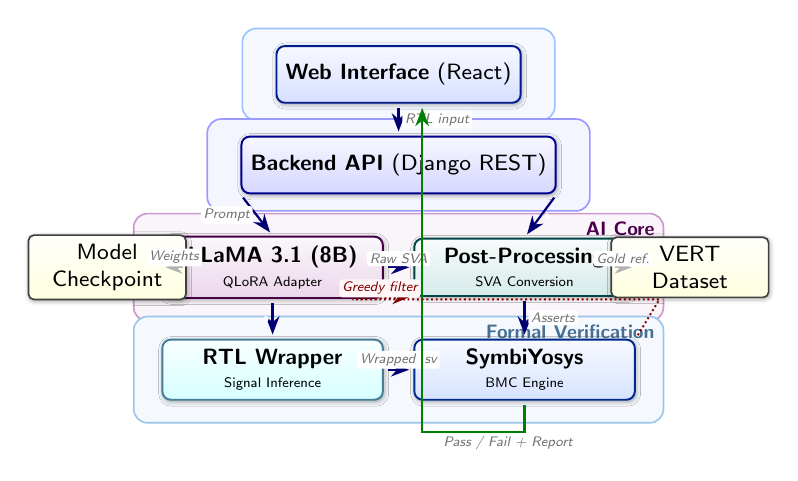
\begin{tikzpicture}[
    >=Stealth,
    % --- Layer background styles ---
    layerbg/.style={rounded corners=5pt, draw=#1!40, line width=0.6pt, fill=#1!4},
    layerlbl/.style={font=\tiny\sffamily\bfseries, text=#1!60!black},
    % --- Component styles ---
    comp/.style={
        draw=#1!55!black, line width=0.7pt, rounded corners=3pt,
        fill=#1!6, top color=#1!3, bottom color=#1!16,
        minimum width=2.8cm, minimum height=0.72cm,
        align=center, font=\footnotesize\sffamily,
        blur shadow={shadow blur steps=5, shadow xshift=0.4pt, shadow yshift=-0.6pt}
    },
    comp/.default=blue,
    store/.style={
        draw=gray!50!black, line width=0.6pt, rounded corners=2pt,
        fill=yellow!5, top color=yellow!2, bottom color=yellow!12,
        minimum width=2.0cm, minimum height=0.6cm,
        align=center, font=\footnotesize\sffamily,
        blur shadow={shadow blur steps=4, shadow xshift=0.3pt, shadow yshift=-0.5pt}
    },
    % --- Arrow styles ---
    flow/.style={->, thick, color=black!55, line width=0.8pt,
        shorten >=1.5pt, shorten <=1.5pt},
    dataflow/.style={->, thick, color=blue!45!black, line width=0.8pt,
        shorten >=1.5pt, shorten <=1.5pt},
    loadarr/.style={->, densely dashed, color=gray!60, line width=0.7pt,
        shorten >=1.5pt, shorten <=1.5pt},
    flbl/.style={font=\tiny\sffamily\itshape, text=black!55, fill=white,
        inner sep=1pt, rounded corners=1pt},
]

% =============================================
%  LAYER 1: Presentation (top)
% =============================================
\node[comp=blue!80!cyan] (ui) at (0, 0) {\textbf{Web Interface} (React)};

% =============================================
%  LAYER 2: API
% =============================================
\node[comp=blue] (api) at (0, -1.15) {\textbf{Backend API} (Django REST)};

% =============================================
%  LAYER 3: AI Core (two columns)
% =============================================
\node[comp=violet] (llm) at (-1.6, -2.45) {\textbf{LLaMA 3.1 (8B)}\\[-1pt]{\tiny QLoRA Adapter}};
\node[comp=teal]   (pp)  at ( 1.6, -2.45) {\textbf{Post-Processing}\\[-1pt]{\tiny SVA Conversion}};

% =============================================
%  LAYER 4: Wrapper + Verification
% =============================================
\node[comp=cyan] (wrap) at (-1.6, -3.75) {\textbf{RTL Wrapper}\\[-1pt]{\tiny Signal Inference}};
\node[comp=blue!70!cyan] (sby) at ( 1.6, -3.75) {\textbf{SymbiYosys}\\[-1pt]{\tiny BMC Engine}};

% =============================================
%  Storage (side)
% =============================================
\node[store] (ckpt) at (-3.7, -2.45) {Model\\Checkpoint};
\node[store] (vert) at ( 3.7, -2.45) {VERT\\Dataset};

% =============================================
%  Layer background boxes
% =============================================
\begin{scope}[on background layer]
    % Presentation layer
    \node[layerbg=blue!60!cyan, fit=(ui), inner xsep=12pt, inner ysep=6pt] (L1) {};
    \node[layerlbl=blue!60!cyan, anchor=west] at (L1.west) {};

    % API layer
    \node[layerbg=blue, fit=(api), inner xsep=12pt, inner ysep=6pt] (L2) {};

    % AI core layer
    \node[layerbg=violet, fit=(llm)(pp), inner xsep=10pt, inner ysep=8pt] (L3) {};
    \node[layerlbl=violet, anchor=north east] at (L3.north east)
         {\scriptsize AI Core};

    % Verification layer
    \node[layerbg=cyan!70!blue, fit=(wrap)(sby), inner xsep=10pt, inner ysep=8pt] (L4) {};
    \node[layerlbl=cyan!70!blue, anchor=north east] at (L4.north east)
         {\scriptsize Formal Verification};
\end{scope}

% =============================================
%  Connections
% =============================================
% Vertical main flow
\draw[dataflow] (ui.south) -- (api.north)
    node[flbl, midway, right, xshift=1pt] {RTL input};
\draw[dataflow] (api.south west) -- (llm.north)
    node[flbl, midway, left, xshift=-1pt] {Prompt};
\draw[dataflow] (llm.east) -- (pp.west)
    node[flbl, midway, above] {Raw SVA};
\draw[dataflow] (pp.south) -- (sby.north)
    node[flbl, midway, right, xshift=1pt] {Asserts};
\draw[dataflow] (api.south east) -- (pp.north)
    node[flbl, midway, right, xshift=1pt] {};
\draw[dataflow] (llm.south) -- (wrap.north)
    node[flbl, midway, left, xshift=-1pt] {};
\draw[dataflow] (wrap.east) -- (sby.west)
    node[flbl, midway, above] {Wrapped .sv};

% Results back up
\draw[flow, color=green!50!black]
    (sby.south) -- ++(0, -0.4) -| ($(ui.south)+(0.3,0)$)
    node[flbl, pos=0.08, below] {Pass / Fail + Report};

% External storage
\draw[loadarr] (ckpt.east) -- (llm.west) node[flbl, midway, above] {Weights};
\draw[loadarr] (vert.west) -- (pp.east) node[flbl, midway, above] {Gold ref.};

% Greedy feedback
\draw[->, densely dotted, thick, color=red!50!black, line width=0.7pt,
      shorten >=1.5pt, shorten <=1.5pt]
    (sby.north east) -- ++(0.3, 0.5) -- ++(-3.9, 0) -- (pp.south west)
    node[flbl, pos=0.45, above, fill=red!3] {\color{red!50!black}Greedy filter};

\end{tikzpicture}
\caption{VISTA system architecture organized in four layers: (1)~the React-based web interface for user interaction, (2)~the Django REST backend for orchestration, (3)~the AI core comprising the fine-tuned LLaMA~3.1 model and SVA post-processing module, and (4)~the formal verification layer with the dynamic RTL wrapper generator and SymbiYosys BMC engine. Dashed arrows indicate static resource loading; the dotted red path shows the greedy syntax feedback loop.}
\label{fig:architecture}
\end{figure}

\begin{itemize}
    \item \textbf{Frontend}: A React-based web interface where users submit RTL designs and view verification results.
    \item \textbf{Backend}: A Django REST API that orchestrates the pipeline, managing prompt construction, model inference, and result aggregation.
    \item \textbf{Core pipeline}: The LLM inference module (using the Unsloth runtime for efficient GPU execution), the assertion post-processing module, the dynamic RTL wrapper generator, and the SymbiYosys formal verification engine.
\end{itemize}

The system achieves end-to-end latency under 25 seconds per RTL fragment on an NVIDIA RTX~4090, dominated by LLM inference time ($\sim$18\,s).

% ============================================================
\section{Challenges and Limitations}
\label{sec:limitations}

\textbf{Don't-care bit patterns.}
RTL constructs using \texttt{casex}/\texttt{casez} with don't-care bits (\texttt{x}, \texttt{z}) cause semantic mismatches in formal equality checks, accounting for the single SBY failure in our evaluation.

\textbf{Temporal operator coverage.}
The current post-processing pipeline converts SVA temporal implications to immediate Boolean assertions, which cannot capture multi-cycle properties (e.g., \texttt{A |\#\#2 B}). This is a deliberate trade-off for Yosys compatibility.

\textbf{Fragment-level evaluation.}
Since VERT provides RTL fragments rather than complete modules, the formal verification validates assertion consistency with the fragment but cannot test assertions against a full design context.

\textbf{Dataset dependence.}
Model performance is bounded by the diversity and quality of the training data. The VERT dataset focuses on conditional and case-based RTL constructs; performance on other RTL idioms (e.g., pipeline stages, memory controllers) requires additional training data.

% ============================================================
\section{Future Work}
\label{sec:future}

Several directions can extend VISTA's capabilities:

\begin{itemize}
    \item \textbf{Counterexample-guided refinement}: Using SymbiYosys counterexample traces to iteratively refine failing assertions through a closed-loop feedback mechanism.
    \item \textbf{Module-level verification}: Extending the wrapper generator to handle complete RTL modules with hierarchical instantiation, enabling verification of inter-module properties.
    \item \textbf{Multi-cycle assertion support}: Integrating formal engines that natively support SVA temporal operators (e.g., Jasper, Questa Formal) to validate sequential properties without conversion to immediate assertions.
    \item \textbf{Reinforcement learning from formal feedback}: Using SBY pass/fail signals as reward signals for RLHF-style training, aligning the model's output distribution toward formally correct assertions.
    \item \textbf{Industrial-scale evaluation}: Testing on larger, industry-standard designs from OpenCores~\cite{opencores} and RISC-V cores to assess scalability.
\end{itemize}

% ============================================================
\section{Conclusion}
\label{sec:conclusion}

We presented VISTA, an end-to-end framework for automated SystemVerilog Assertion generation from RTL code using a fine-tuned LLaMA~3.1~(8B) model. By combining domain-specific QLoRA fine-tuning, a dynamic RTL wrapping template, and a multi-stage assertion post-processing pipeline, VISTA achieves 99\% formal verification pass rate and 99.1\% Jaccard similarity to gold-standard assertions on 100 VERT test samples. Our ablation study demonstrates that prompt--training alignment and clock-aware wrapper generation are the two most critical factors for achieving high accuracy. VISTA demonstrates that large language models, when tightly integrated with formal verification methodology, can substantially automate assertion-based hardware verification, reducing the manual effort that constitutes a major bottleneck in modern SoC design flows.

% ============================================================
\balance
\bibliographystyle{IEEEtran}
\begin{thebibliography}{20}

\bibitem{foster2015trends}
H.~Foster, ``Trends in functional verification: A 2014 industry study,'' in \emph{Proc.\ Design Automation Conf.\ (DAC)}, 2015, pp.~1--6.

\bibitem{ieee1800}
IEEE Standards Association, ``IEEE Standard for SystemVerilog---Unified Hardware Design, Specification, and Verification Language,'' \emph{IEEE Std 1800-2023}, 2023.

\bibitem{goldmine}
S.~Vasudevan, D.~Sheridan, S.~Patel, D.~Tcheng, B.~Tuohy, and D.~Johnson, ``GoldMine: Automatic assertion generation using data mining and static analysis,'' in \emph{Proc.\ Design, Automation and Test in Europe (DATE)}, 2010, pp.~626--629.

\bibitem{harm}
S.~Vasudevan \emph{et~al.}, ``HARM: Hardware assertion and RTL mining,'' in \emph{Proc.\ DAC}, 2013, pp.~1--6.

\bibitem{spec2assertion}
``Spec2Assertion: Automatic Pre-RTL Assertion Generation by LLMs,'' \emph{arXiv:2505.07995}, 2025.

\bibitem{assertllm}
A.~D'Souza, ``AssertLLM: Advancing Hardware Verification with AI,'' LinkedIn, Feb.\ 2025.

\bibitem{assertionforge}
NVlabs/AssertionForge, GitHub Repository, Jun.\ 2025.

\bibitem{assertionbench}
M.~Halpern \emph{et~al.}, ``AssertionBench: A Benchmark to Evaluate Large-Language Models for Assertion Generation,'' \emph{arXiv:2406.18627}, Jun.\ 2024.

\bibitem{enhancing_llm_hw}
``Enhancing Large Language Models for Hardware Verification,'' \emph{arXiv:2503.08923}, Mar.\ 2025.

\bibitem{qlora}
T.~Dettmers, A.~Pagnoni, A.~Holtzman, and L.~Zettlemoyer, ``QLoRA: Efficient Finetuning of Quantized Language Models,'' \emph{arXiv:2305.14314}, May 2023.

\bibitem{unsloth}
Unsloth.ai Documentation, \url{https://unsloth.ai}, 2025.

\bibitem{vert}
``VERT: Verified RTL-to-SVA Dataset,'' \emph{GitHub/HuggingFace}, 2024.

\bibitem{symbiyosys}
SymbiYosys Documentation, \url{https://symbiyosys.readthedocs.io}, accessed Apr.\ 2026.

\bibitem{sva_basics}
``SystemVerilog Assertions Basics,'' \url{https://systemverilog.io}, accessed Apr.\ 2026.

\bibitem{opencores}
OpenCores.org RTL Modules Archive, \url{https://opencores.org}, accessed Apr.\ 2026.

\end{thebibliography}

\end{document}
